\section{Evaluation}\label{sec:evaluation}\vspace{-2pt}

% \begin{table}[]
\centering
\begin{tabular}{|c|c|c|c|c|c|}
\hline
\textbf{} &
  \textbf{Scenario Description} &
  \textbf{Poke} &
  \textbf{Push} &
  \textbf{Grasp}\\ \hline
\textbf{S1} & No Obstacles & \checkmark & \checkmark & \checkmark \\ \hline
\textbf{S2} & 2 Obstacles  & \checkmark & \checkmark & \checkmark \\ \hline
\textbf{S3} & 4 Obstacles  & \checkmark & \checkmark & \checkmark \\ \hline
\textbf{S4} & Wide Object  & \checkmark & \checkmark & \\ \hline
\textbf{S5} & Tunnel       & \checkmark &  & \checkmark \\ \hline
\textbf{S6} & Shared Workspace & \checkmark & & \\ \hline
\end{tabular}
\caption{We evaluate PokeRRT* in 6 different scenarios and demonstrate its superiority to pushing and pick-and-place in S4, S5, and S6. See \cref{fig:scenarios} for visualizations of these test conditions.\vspace{-17pt}}
\label{tab:scenarios}
\end{table}

In this section, we qualitatively and quantitatively evaluate \textsl{PokeRRT} and \textsl{PokeRRT*} in simulation and the real-world under various environment setups.\footnote{Links to our code, videos, and demonstrations of the experiments are available here: \href{https://hiro-group.ronc.one/poke-rrt-icra-22.html}{https://hiro-group.ronc.one/poke-rrt-icra-22.html}.} We measure success rates, task times (in seconds), and number of executed actions in the final planned path for both motion planners. Success rates are averaged across all scenarios for a given planner, whereas task times and number of executed actions are presented separately for each scenario. Task time is defined as the sum of planning, execution, and replanning times. Object start pose is kept fixed across various trials to aid reproducibility of results. Simulation and real-world results are averaged over 250 and 10 trials, respectively.
%
Collectively, our results demonstrate that \textsl{PokeRRT} and \textsl{PokeRRT*} indeed enable fast and successful manipulation of objects in conditions where push planning and pick-and-place fail.

\subsection{Experimental Setup}

\begin{table*}[]
\vspace{4pt}
\resizebox{\textwidth}{!}{
\centering
\begin{tabular}{c|c|c|c|c|c|c|c|}
\cline{2-8}
 &
  \multicolumn{6}{c|}{\textbf{Task Time [seconds]}}&\multicolumn{1}{c|}{\textbf{Success Rate}}\\ \hline
\multicolumn{1}{|c|}{\textbf{Planner}} &
  \textbf{S1} &
  \textbf{S2} &
  \textbf{S3} &
  \textbf{S4} &
  \textbf{S5} &
  \textbf{S6} 
  & \textbf{S1 - S6}\\ \hline
\multicolumn{1}{|c|}{PokeRRT*} & 
\textbf{46.43 (21.67)} & 
212.74 (100.01) & 
232.42 (118.63) & 
70.47 (38.82) & 
132.62 (98.27) & 
\textbf{130.01 (84.05)} & 
0.87 (0.31) \\ \hline
\multicolumn{1}{|c|}{PokeRRT} & 
49.69 (21.11) & 
\textbf{196.54 (124.61)} & 
\textbf{167.55 (138.63)} & 
\textbf{64.14 (52.45)} & 
\textbf{116.35 (89.72)}& 
171.77 (103.21) & 
\textbf{0.88 (0.31)} \\ \hline
\multicolumn{1}{|c|}{\begin{tabular}[c]{@{}c@{}}LI-PokeRRT*\end{tabular}} & 
169.87 (71.28) & 
378.90 (122.21) & 
346.70 (111.71) & 
165.91 (44.87) & 
N/A & 
N/A & 
0.53 (0.28) \\ \hline
\multicolumn{1}{|c|}{\begin{tabular}[c]{@{}c@{}}LI-PokeRRT\end{tabular}} & 
123.71 (36.72) & 
328.66 (107.18) & 
322.28 (138.05) &
135.80 (32.91) & 
N/A & 
N/A & 
0.63 (0.18) \\ \hline
\multicolumn{1}{|c|}{\begin{tabular}[c]{@{}c@{}}Push Planner\end{tabular}} & 
122.68 (47.07) & 
284.78 (104.40) & 
249.32 (68.30) & 
117.58 (67.05) & 
N/A & 
N/A & 
0.44 (0.26) \\ \hline\hline
\multicolumn{1}{|c|}{Pick-and-Place} & 
16.29 (3.76) & 
17.71 (3.81) & 
16.14 (3.25) & 
N/A & 
19.15 (4.99) & 
N/A & 
0.67 (0.00)\\ \hline
\end{tabular}
}
\caption{Task times [\textsl{mean (stddev)}] for various planning algorithms in simulation are presented. Success rates are aggregated across all 6 scenarios. Overall, poke planning is faster than push planning and leads to higher success rate than pushing or grasping. Low-impulse (LI) poke planners and the push planner are unsuccessful in S5 and S6 due to action path collisions (S5) or goal region being outside the robot's reachable workspace (S6). The robot is unable to pick or place object in S4 and S6  due to limitations in robot mechanics.\vspace{-12pt}}
\label{tab:eval-sim-time}
\end{table*}

\subsubsection{Scenarios}\label{sec:evaluation-scenarios}

We test multiple algorithms for poking, pushing, and grasping manipulation in six scenarios (\cref{fig:scenarios}).
% \ap{\textsl{PokeRRT} and \textsl{PokeRRT*} expand a robot's reachable workspace, in contrast to pushing and pick-and-place which operate within this region. Pushing also operates under the quasistatic assumption, as a result of which the robot must maintain constant contact with the object. And finally, pick-and-place is also limited by the object dimensions, i.e., if the object is bigger than the gripper width, pick-and-place will fail.}
Our motivating application is the concurrent operation of two robots with potentially non-overlapping reachable regions located in adjacent workcells on a factory floor. Therefore, the objects being manipulated must be accessible by both robots to enable successful collaboration.
Given this motivation, scenarios are designed to test the flexibility of the planner in generating plans for manipulating the object in a planar workspace from a fixed start pose to a goal region, which represents the workspace of a second robot. To ensure that object--obstacle collisions are handled robustly through the replanning strategy, we enforce the following properties in our scenarios: i) the objects used in each scenario are rigid and therefore retain their shape across multiple trials and ii) obstacles are fixed to the table so that collisions do not change the planning configuration space.

Scenarios 1-3 (S1-S3 in \cref{fig:scenarios}) are designed to test baseline manipulation capability through uncluttered (S1) and cluttered (S2, S3) environments. S2 and S3 contain 2 and 4 obstacles, respectively, at fixed poses in the shared robot workspace. The object being manipulated has size $[9, 14, 5]$ cm and mass $m=87$ g. Poke planning, push planning, and pick-and-place will all work in these scenarios since the goal region overlaps with the first robot's reachable workspace.
Scenario 4 (S4 in \cref{fig:scenarios}) contains a bigger cuboid object of size $[11, 18, 11]$ cm and mass $m=112$ g in an obstacle-free workspace. Poke planning and push planning will work in this scenario, however pick-and-place will not since gripper width ($10$ cm) is smaller than the minimum dimension of the cuboid. This scenario represents situations where object properties are incompatible with robot kinematics, i.e., if the object of interest is too heavy or too wide to be grasped or if the end-effector is malfunctional, and the robot needs to formulate an alternate manipulation plan.

Scenario 5 (S5 in \cref{fig:scenarios}) presents two work cells with a tunnel in the center of the table. The first robot cannot push the object to the second robot because the end-effector will collide with the divider along its action path. However, poke planning will succeed due to the short duration of robot--object contact. The first robot is able to grasp the object over the divider in our setup but for larger dividers such as a screen, pick-and-place will fail.
Scenario 6 (S6 in \cref{fig:scenarios}) contains an obstacle-free workspace with non-overlapping reachable regions for each robot. The first robot is able to poke the target object to the second robot's reachable workspace, but cannot push or pick-and-place due to limited reachability. Since pushing operates under the quasitstatic assumption, it requires constant contact between the robot end-effector and the object being manipulated and therefore, manipulation is limited by robot kinematics and reachability. This scenario represents cases where task success is limited by the robot's kinematic characteristics, i.e., if the goal pose is outside the robot's reachable workspace.

\subsubsection{Parameters}

The action vector $\boldsymbol{a_{valid}} = \langle \boldsymbol{p_c}, \boldsymbol{\|\vec{v}_{EE}\|}\rangle$ for our proposed motion planners is generated at runtime. Contour points $p_c$ close to object corners are ignored for clean pokes. The velocity magnitudes $\|\vec{v}_{EE}\|$ are sampled in the $[0.3, 1.0]$ m/s range to increase likelihood of robot joints achieving the commanded operational space velocities. Goal region is defined as the workspace of the second robot, determined as the frequency of inverse kinematics poses achievable on discretized xy-locations on the planar support surface of the object. The empirically-determined replanning threshold is $5cm$ and $10^{\circ}$.

\subsubsection{Algorithms}

\textsl{PokeRRT} and \textsl{PokeRRT*} are compared against several baseline approaches. To evaluate pushing, we use the \textsl{Two-Level Push Planner} presented in \cite{zito2012two} since it also uses simulation in the planning loop to get the next feasible environment state. This work integrates simulation-based forward modeling with sampling-based motion planning to explore the space of feasible pushing actions required to get an object from start to goal. Our baseline approaches, \textsl{Low-Impulse (LI) PokeRRT} and \textsl{Low-Impulse (LI) PokeRRT*}, are designed to show that poking is a more fundamental manipulation skill and encompasses pushing if the applied impulse magnitudes are kept small. They operate similarly to \textsl{PokeRRT} and \textsl{PokeRRT*} but with $\|\vec{v}_{EE}\| = 0.2$ m/s to simulate pushing. Any replanning for a given planner is done using that same planner. Lastly, \textsl{Pick-and-Place} is performed in an open-loop manner with predefined grasps for known objects. An experimental trial fails if the planner does not find a valid plan to the goal region in 240 seconds or if the object falls off the table during execution.\vspace{-4pt}

\begin{table}[]
\resizebox{\columnwidth}{!}{
\centering
\begin{tabular}{c|c|c|c|c|c|c|}
\cline{2-7}
                                                                                     & \multicolumn{6}{c|}{\textbf{Number of Actions in Execution Path}}                                 \\ \hline
\multicolumn{1}{|c|}{\textbf{Planner}}                                               & \textbf{S1} & \textbf{S2} & \textbf{S3} & \textbf{S4} & \textbf{S5} & \textbf{S6} \\ \hline
\multicolumn{1}{|c|}{PokeRRT*}                                                       & 
\textbf{\begin{tabular}[c]{@{}c@{}}3.93\\ (0.98)\end{tabular}} & \textbf{\begin{tabular}[c]{@{}c@{}}4.62\\ (1.04)\end{tabular}}                       
&   \textbf{\begin{tabular}[c]{@{}c@{}}4.49\\ (1.02)\end{tabular}}   
&   \textbf{\begin{tabular}[c]{@{}c@{}}4.76\\ (1.20)\end{tabular}}   
& \textbf{\begin{tabular}[c]{@{}c@{}}3.71\\ (1.02)\end{tabular}} &  \textbf{\begin{tabular}[c]{@{}c@{}}3.65\\ (1.08)\end{tabular}}\\ \hline
\multicolumn{1}{|c|}{PokeRRT} &
  \begin{tabular}[c]{@{}c@{}}6.10 \\ (1.96)\end{tabular} &
\begin{tabular}[c]{@{}c@{}}8.21\\ (2.95)\end{tabular}  &
\begin{tabular}[c]{@{}c@{}}7.94\\ (2.08)\end{tabular}  &\begin{tabular}[c]{@{}c@{}}6.77\\ (2.35)\end{tabular}
  &
\begin{tabular}[c]{@{}c@{}}4.56\\ (1.27)\end{tabular}  &
 \begin{tabular}[c]{@{}c@{}}8.17\\ (2.46)\end{tabular} \\ \hline
\multicolumn{1}{|c|}{\begin{tabular}[c]{@{}c@{}}LI-PokeRRT*\end{tabular}} & 
\begin{tabular}[c]{@{}c@{}}16.43\\ (2.28)\end{tabular}&
\begin{tabular}[c]{@{}c@{}}22.27\\ (2.26)\end{tabular}
&\begin{tabular}[c]{@{}c@{}}19.00\\ (1.54)\end{tabular}
&\begin{tabular}[c]{@{}c@{}}18.54\\ (1.44)\end{tabular}
&N/A
& N/A            \\ \hline

\multicolumn{1}{|c|}{\begin{tabular}[c]{@{}c@{}}LI-PokeRRT\end{tabular}} &
\begin{tabular}[c]{@{}c@{}}19.08 \\ (1.51)\end{tabular}
  &
\begin{tabular}[c]{@{}c@{}}19.62\\ (1.64)\end{tabular}  &
 \begin{tabular}[c]{@{}c@{}}20.74\\ (2.13)\end{tabular} &\begin{tabular}[c]{@{}c@{}}19.38\\ (1.59)\end{tabular}
  &
N/A  &
N/A  \\ \hline
\multicolumn{1}{|c|}{\begin{tabular}[c]{@{}c@{}}Push Planner\end{tabular}} &
\begin{tabular}[c]{@{}c@{}}8.72 \\ (1.42)\end{tabular} &
\begin{tabular}[c]{@{}c@{}}8.61\\ (1.71)\end{tabular}   &
\begin{tabular}[c]{@{}c@{}}7.68\\ (1.19)\end{tabular}   &\begin{tabular}[c]{@{}c@{}}8.53 \\ (1.51)\end{tabular}
  &N/A
   &N/A
   \\ \hline\hline
\multicolumn{1}{|c|}{Pick-and-Place}                                                 & \begin{tabular}[c]{@{}c@{}}1.00\\ (0.00)\end{tabular}           & \begin{tabular}[c]{@{}c@{}}1.00\\ (0.00)\end{tabular}           & \begin{tabular}[c]{@{}c@{}}1.00\\ (0.00)\end{tabular}           & N/A           & \begin{tabular}[c]{@{}c@{}}1.00\\ (0.00)\end{tabular}           & N/A           \\ \hline
\end{tabular}
}
\caption{Number of executed actions in the planned path for various algorithms in simulation are presented here. Both \textsl{PokeRRT*} and  \textsl{Low-Impulse PokeRRT*} lead to fewer actions than their RRT-based counterparts, thus exploiting the large displacement property inherent to poking manipulation.\vspace{-12pt}}
\label{tab:eval-sim-actions}
\end{table}

\subsection{Simulation Experiments}

\cref{tab:eval-sim-time} shows the task times and success rates for \textsl{Pick-and-Place} and five non-prehensile manipulation planners---\textsl{PokeRRT*},  \textsl{Low-Impulse PokeRRT*},  \textsl{PokeRRT},  \textsl{Low-Impulse PokeRRT}, and \textsl{Two-Level Push Planner}. Results are averaged over 250 trials. \textsl{PokeRRT} and \textsl{PokeRRT*} successful in all scenarios while \textsl{Two-Level Push Planner} fails in S5 and S6 and grasping fails in S4 and S6. \textsl{Two-Level Push Planner} has a low overall success rate ($44\%$), as expected based on the reasons presented in \cref{sec:evaluation-scenarios}.

\textsl{PokeRRT} and \textsl{PokeRRT*} task times are lower than \textsl{Two-Level Push Planner} task times across all scenarios. Standard deviations are high due to the sampling-based nature of our planners. The task time for S4 is greater than for S1 since the object used in S4 is not only bigger in size but also larger in mass than the object used in S1, therefore poke displacements are lower given the same contact force. \textsl{Pick-and-Place} has the lowest task time because it does not involve planning in the object configuration space---the robot moves to object pose, grasps, and moves to goal pose, so only a single action is executed. Low-impulse poke planners have large search trees due to shorter displacements of the object. This results in longer planning times and also lower success rates. Task times are higher for obstacle scenarios because the robot end-effector is more likely to run into obstacles and collision checking is a computationally expensive procedure.

\textsl{Pick-and-Place} succeeds in simulation for S1, S2, S3, and S5 because there is no uncertainty in object pose so manipulation consists of moving to a predefined grasp configuration and moving to the goal pose. We intentionally set up the start and goal configurations for \textsl{Pick-and-Place} to create an upper bound for comparison with our planners. For the reasons presented in \cref{sec:evaluation-scenarios}, it fails in S4 and S6. Low-impulse poke planners have higher success rates than the push planner because the shorter robot control trajectories corresponding to poking result in fewer obstacle collisions. Low-impulse poke planners fail in S5 and S6 because the pokes are not strong enough to pass the workspace divider or cross into the second robot's reachable workspace.

% \begin{figure}
%   \centering
%     \includegraphics[width=\linewidth]{figures/sampleplans}
%   \caption{Plans generated by \textsl{PokeRRT} (a) involve more pokes than those generated by \textsl{PokeRRT*} (b), which indicates that \textsl{PokeRRT*} is better able to exploit poking's key characteristic of covering large distances.\vspace{-28pt}}\label{fig:plans}
% \end{figure}
% \vspace{-4.5pt}
\cref{tab:eval-sim-actions} presents the number of executed actions in the final planned path for multiple planning algorithms across several scenarios. It indicates that the number of executed actions is lower for \textsl{PokeRRT} and \textsl{PokeRRT*} compared to \textsl{Two-Level Push Planner}, showing that poke planners can displace the object further with fewer actions in less time. Notably, the number of actions is lowest for \textsl{PokeRRT*}, thereby supporting our claim that minimizing the number of poking actions exploits the large displacement property of poking manipulation.
% (\cref{fig:plans}).
However, the task time is similar to that of \textsl{PokeRRT} since \textsl{PokeRRT*} introduces the choose parent and rewiring steps to \textsl{PokeRRT}, which increases the number of actions sampled while planning. In general, \textsl{PokeRRT} is preferable in scenarios with obstacles---even though the number of pokes for \textsl{PokeRRT*} is lower (i.e., faster overall execution), a greater percentage of time is spent on resampling actions in \textsl{PokeRRT*}, most of which lead to object--obstacle collisions. Task times for low-impulse poke planners are comparable to \textsl{Two-Level Push Planner}, supporting our claim that pushing is a limiting case of poking where applied impulses are low in magnitude.

\begin{figure}
\vspace{4pt}
  \centering
    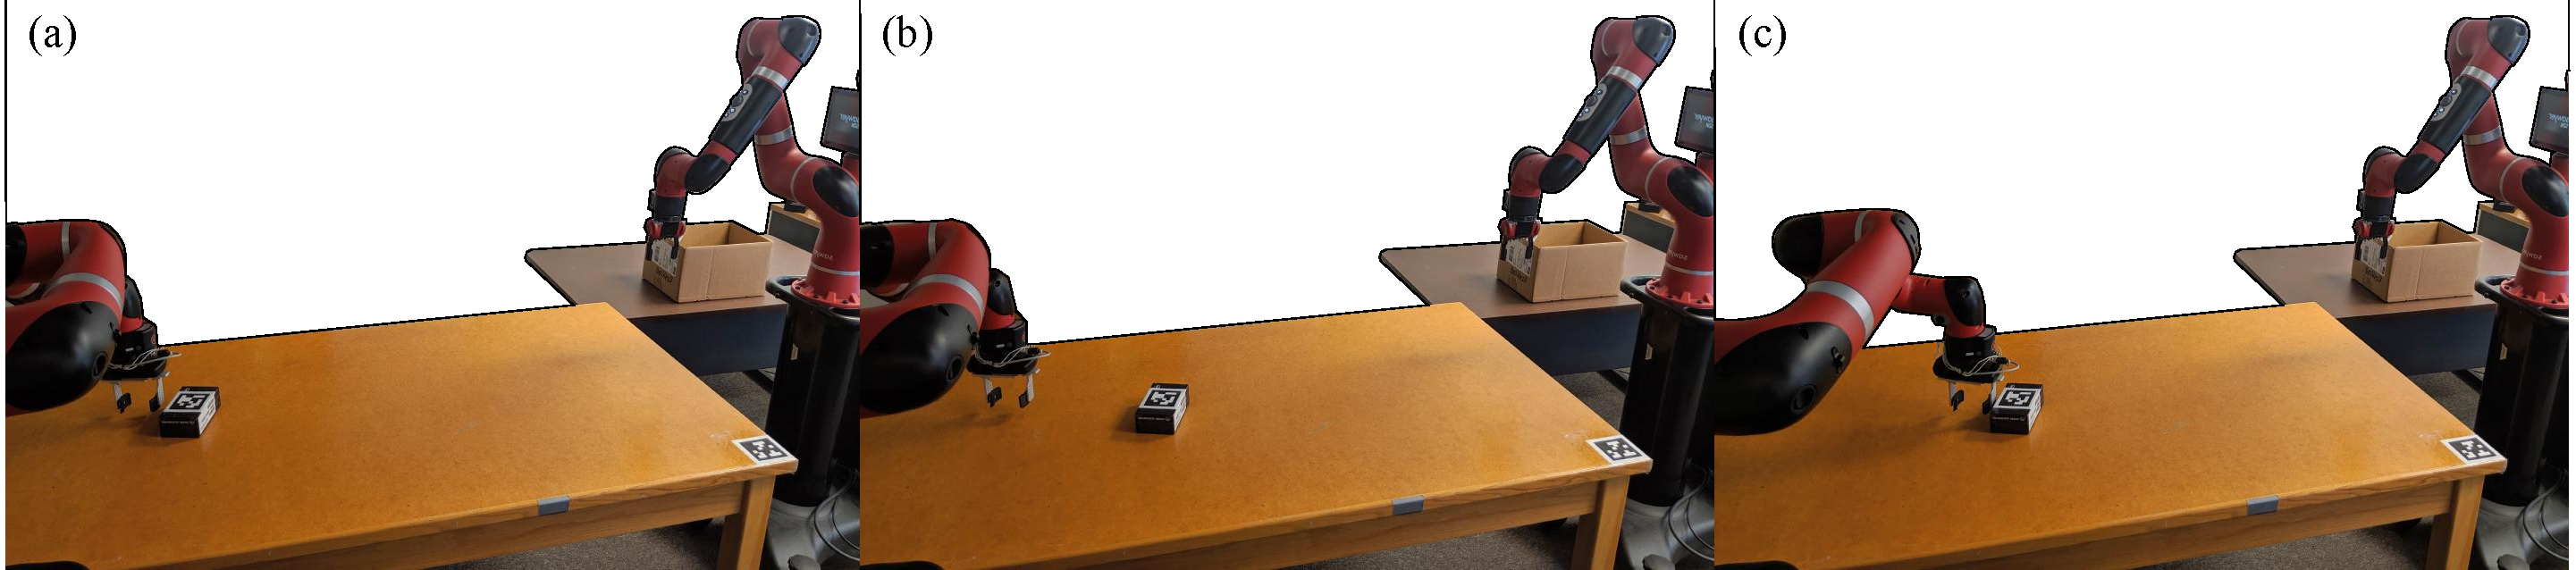
\includegraphics[width=\linewidth]{figures/vignette1-min.pdf}\\
    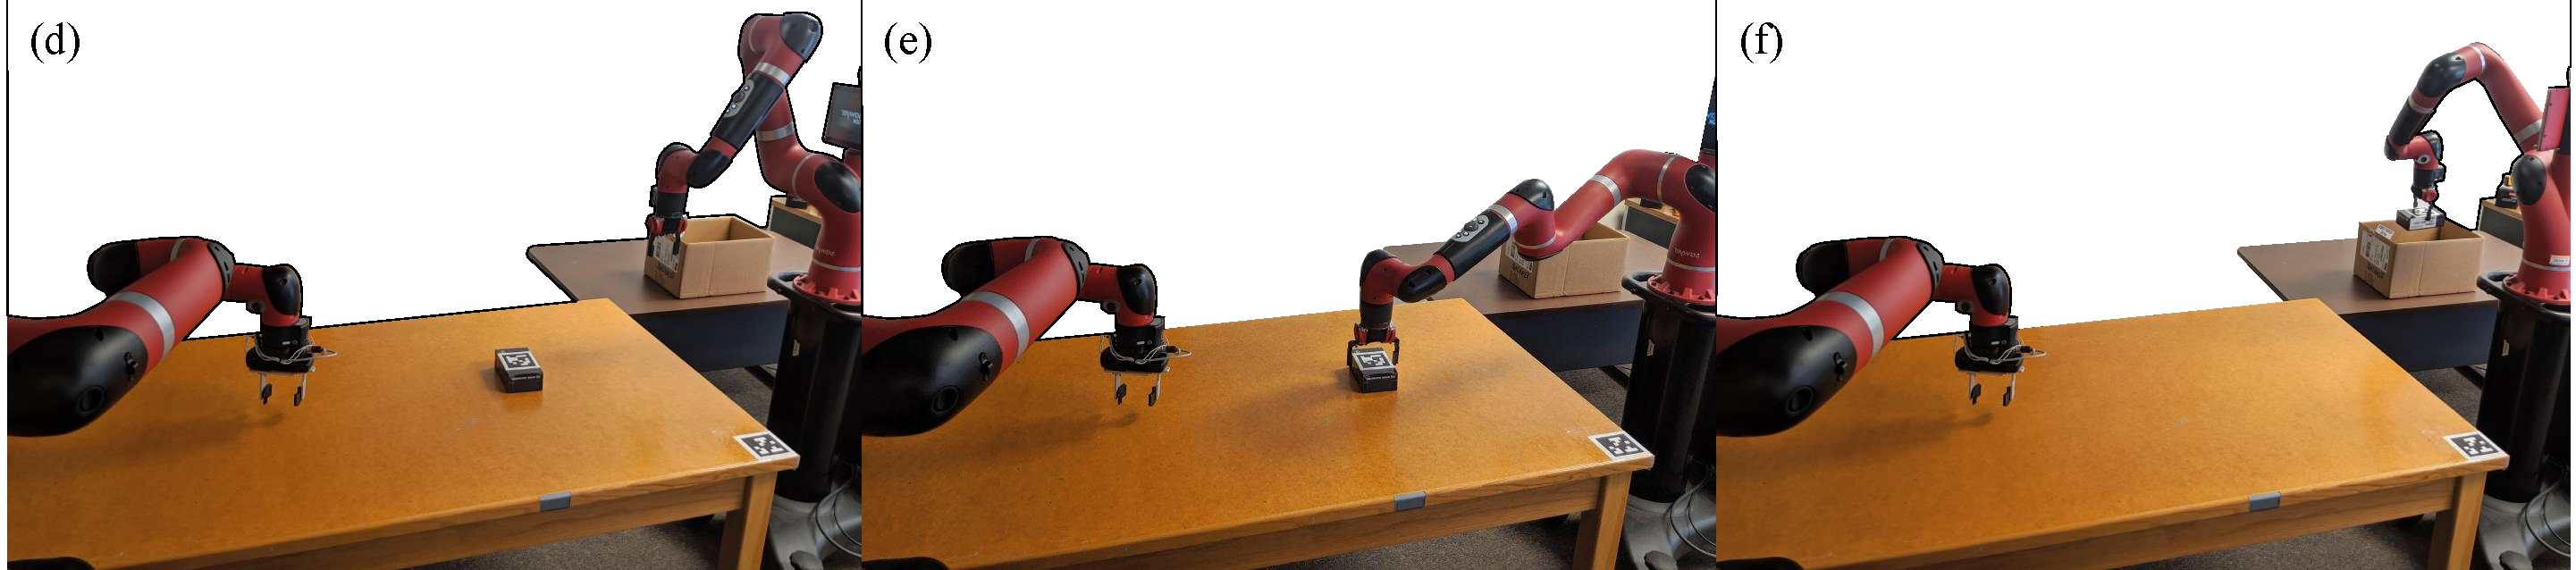
\includegraphics[width=\linewidth]{figures/vignette2-min.pdf}
  \vspace{-12pt}
  \caption{Two robots with non-overlapping reachable regions are shown (S6). Robot A (left) applies 2 pokes to manipulate the object to Robot B's (right) workspace (a-d). Robot B then grasps the object and places it in a bin that is not reachable by Robot A (e-f).\vspace{-15pt}}\label{fig:vignette}
\end{figure}

\subsection{Real-World Experiments}

We evaluate \textsl{PokeRRT*}, \textsl{PokeRRT}, \textsl{Two-Level Push Planner}, and \textsl{Pick-and-Place} for a subset of the scenarios in the real-world (\cref{tab:eval-real}). The task times and the number of actions executed in the real world are slightly higher than in simulation. This is expected because the plan is generated in simulation and simulation does not fully capture the complexities of the real-world environment. Therefore, replanning is required for real-world plan execution which leads to an increase in task times. As shown in \cref{fig:plot}, execution times for poke planners are lower than for the push planner indicating that poke planning leads to faster object manipulation than push planning. Additionally, the replanning time for push planning is higher than for poke planning since simulating push actions to generate the planning graph takes more computational cycles than simulating instantaneous contact for poke actions. However, the number of replans for push planning is lower than for poke planning thereby pointing to the inherently uncontrollable nature of poking, which may not be desirable in certain situations (\cref{tab:eval-real}).
Collectively, real-world results align with the results from simulation.
% Similar to simulation results, \textsl{PokeRRT*} has the fewest number of executed actions. In S4, poking is 1.7 times faster than pushing. In S5, pushing fails because of collision with obstacles and grasping fails because the object is too large for the gripper. Both pushing and grasping fail in S6 because the goal region is unreachable.

\cref{fig:vignette} depicts a failure recovery case for S6 where failure to grasp or push to the second robot's reachable workspace does not result in task failure---the first robot pokes the object to the second robot's reachable workspace, allowing the second robot to successfully manipulate the object.
Additionally, while grasping is a faster form of manipulation with fewer actions than poking or pushing, it has a lower overall success rate ($27\%$) than pushing ($33\%$) due to perception inaccuracies. This discrepancy between simulation and real-world results points to a fundamental difference between grasping and poking or pushing---sensing uncertainty leads to total failure in grasping, whereas for poking it leads to just partial failure as our presented planners operate in a closed-loop manner. 


% Please add the following required packages to your document preamble:
% \usepackage{multirow}
% \begin{table*}[]
% \vspace{4pt}
% \resizebox{\textwidth}{!}{
% \centering
% \begin{tabular}{c|c|c|c|c|c|c|c|}
%   \cline{2-8}
%   &
%   \multicolumn{3}{c|}{\textbf{Task Time [seconds]}} &
%   \multicolumn{3}{c|}{\textbf{Number of Actions}} &
%   \multicolumn{1}{c|}{\textbf{Success Rate}} \\ \hline
%   \multicolumn{1}{|c|}{\textbf{Planner}} &
%   \textbf{S4} &
%   \textbf{S5} &
%   \textbf{S6} &
%   \textbf{S4} &
%   \textbf{S5} &
%   \textbf{S6} &
%   \textbf{S4 - S6} \\ \hline
% \multicolumn{1}{|c|}{PokeRRT*} &
%   \textbf{69.58 (26.15)} &
%   \textbf{127.45 (57.80)} &
%   182.03 (122.77) &
%   \textbf{5.27 (2.00)} &
%   \textbf{5.12 (1.05)} &
%   \textbf{6.11 (1.91)} &
%   \textbf{0.9 (0.3)} \\ \hline
% \multicolumn{1}{|c|}{PokeRRT} &
%   83.55 (29.59) &
%   148.55 (86.23) &
%   \textbf{157.03 (94.41)} &
%   6.20 (1.60) &
%   6.67 (1.56) &
%   6.88 (2.15) &
%   \textbf{0.9 (0.3)}\\ \hline
% \multicolumn{1}{|c|}{Two-Level Push Planner} &
%   120.21 (47.09) &
%   N/A &
%   N/A &
%   6.00 (1.26) &
%   N/A &
%   N/A &
%   0.33 (0.47) \\ \hline\hline
% \multicolumn{1}{|c|}{Pick-and-Place} &
%   N/A &
%   20.31 (3.21) &
%   N/A &
%   N/A &
%   1.00 (0.00) &
%   N/A &
%   0.27 (0.44) \\ \hline
% \end{tabular}
% }
% \caption{Real-world task times, number of actions in executed path, and success rates are presented in this table. Results are averaged across 10 trials. Pushing has the highest success rate and fastest task times. PokeRRT* generates plans with the fewest number of actions.\vspace{-14pt}}
% \label{tab:eval-real}
% \end{table*}

\begin{table*}[]
\vspace{4pt}
\centering\small
\resizebox{0.95\textwidth}{!}{
\centering
\begin{tabular}{|c|c|c|c|c|c|}
  \hline
   \textbf{Planner} & & PokeRRT* & PokeRRT & Two-Level Push Planner & Pick-and-Place \\
   \hline
  \multirow{3}{*}{\textbf{Task Time [seconds]}} & \textbf{S4} & \textbf{69.58 (26.15)} & 83.55 (29.59) & 120.21 (47.09) & N/A \\ \cline{2-6}
  & \textbf{S5} & \textbf{127.45 (57.80)} & 148.55 (86.23) & N/A & 20.31 (3.21) \\ \cline{2-6}
  & \textbf{S6} & 182.03 (122.77) & \textbf{157.03 (94.41)} & N/A & N/A \\ \hline
  \multirow{3}{*}{\textbf{Number of Actions}} & \textbf{S4} & \textbf{5.27 (2.00)} & 6.20 (1.60) & 6.00 (1.26) & N/A \\ \cline{2-6}
  & \textbf{S5} & 5.12 (1.05) & 6.67 (1.56) & N/A & \textbf{1.00 (0.00)} \\ \cline{2-6}
  & \textbf{S6} & \textbf{6.11 (1.91)} & 6.88 (2.15) & N/A & N/A \\ \hline
%   \multirow{3}{*}{\textbf{Initial Planning Time}} & \textbf{S4} & 4.64 (1.70) & 7.19 (7.26) & 19.10 (8.66) & N/A \\ \cline{2-6} 
%   & \textbf{S5} & 18.95 (12.41) & 29.97 (31.22) & N/A & N/A \\ \cline{2-6}
%   & \textbf{S6} & 15.38 (14.35) & 22.91 (34.66) & N/A & N/A \\ \hline
  \multirow{3}{*}{\textbf{Number of Replans}} & \textbf{S4} & 3.45 (1.67) & 4.2 (1.6) & \textbf{2.80 (1.54)} & N/A \\ \cline{2-6} 
  & \textbf{S5} & \textbf{3.38 (1.32)} & 4.11 (1.37) & N/A & N/A \\ \cline{2-6}
  & \textbf{S6} & \textbf{4.22 (1.81)} & 4.38 (1.49) & N/A & N/A \\ \hline
%   \multirow{3}{*}{\textbf{Replanning Times}} & \textbf{S4} & 4.75 (1.72) & 3.4 (2.01) & 10.04 (4.56) & N/A \\ \cline{2-6} 
%   & \textbf{S5} & 16.42 (9.89) & 11.58 (10.79) & N/A & N/A \\ \cline{2-6}
%   & \textbf{S6} & 22.56 (19.65) & 11.28 (10.32) & N/A & N/A \\ \hline
%   \multirow{3}{*}{\textbf{Execution Time}} & \textbf{S4} & 9.21 (0.5) & 9.53 (0.86) & 11.16 (0.46) & N/A \\ \cline{2-6} 
%   & \textbf{S5} & 9.47 (0.48) & 9.11 (0.28) & N/A & N/A \\ \cline{2-6}
%   & \textbf{S6} & 8.84 (0.23) & 10.20 (1.70) & N/A & N/A \\ \hline
  \textbf{Success Rate} & \textbf{S4 - S6} & \textbf{0.9 (0.3)} & \textbf{0.9 (0.3)} & 0.33 (0.47) & 0.27 (0.44)\\ \hline
\end{tabular}
}
\caption{Real-world task times, number of actions in executed path, and success rates are presented in this table. Results are averaged across 10 trials. Pushing has the highest success rate and fastest task times. PokeRRT* generates plans with the fewest number of actions.\vspace{-12pt}}
\label{tab:eval-real}
\end{table*}

\begin{figure}
\vspace{4pt}
  \centering
    \hspace{-7pt}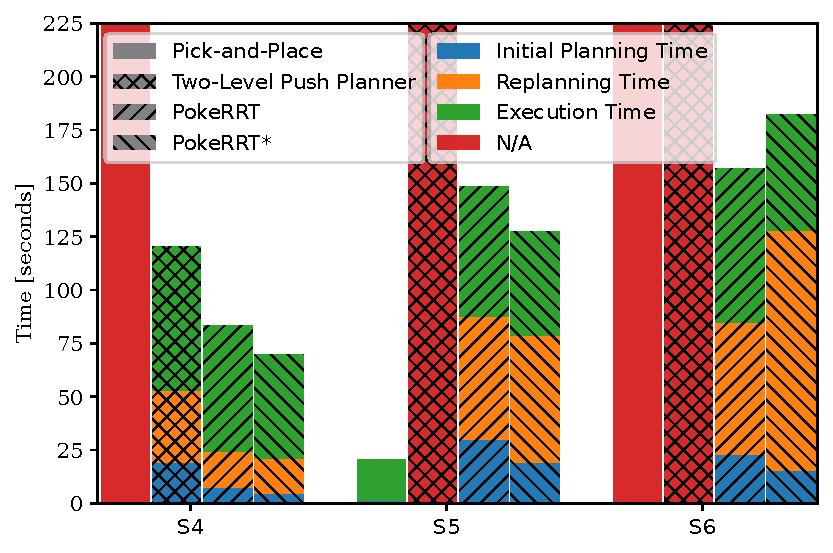
\includegraphics[width=\linewidth]{figures/plot.pdf}
%   \vspace{-12pt}
  \caption{A breakdown of task time as the sum of initial planning, replanning, and execution times is presented for various planners in the real-world. A single bar indicates total task time. Long red bars indicate cases where tasks cannot be solved. Overall, poke planning demonstrates lower execution and replanning times than push planning. \vspace{-10pt}}\label{fig:plot}
\end{figure}

